% !TEX TS-program = pdflatex
% !TEX encoding = UTF-8 Unicode

% This is a simple template for a LaTeX document using the "article" class.
% See "book", "report", "letter" for other types of document.

\documentclass[11pt]{article} % use larger type; default would be 10pt.
\setcounter{secnumdepth}{2}

\usepackage{paralist} % very flexible & customisable lists (eg. enumerate/itemize, etc.)

\usepackage[utf8]{inputenc} % set input encoding (not needed with XeLaTeX)
\usepackage{float} % to place float images correctly
\usepackage{color} % to color text
\usepackage{enumitem} % for lists
\usepackage{subfigure} % for mockups

%%% Examples of Article customizations
% These packages are optional, depending whether you want the features they provide.
% See the LaTeX Companion or other references for full information.

%%% PAGE DIMENSIONS
\usepackage{geometry} % to change the page dimensions
\geometry{a4paper} % or letterpaper (US) or a5paper or....
% \geometry{margin=2in} % for example, change the margins to 2 inches all round
% \geometry{landscape} % set up the page for landscape
%   read geometry.pdf for detailed page layout information

\usepackage{graphicx} % support the \includegraphics command and options

% \usepackage[parfill]{parskip} % Activate to begin paragraphs with an empty line rather than an indent

%%% PACKAGES
\usepackage{booktabs} % for much better looking tables
\usepackage{array} % for better arrays (eg matrices) in maths
%\usepackage{paralist} % very flexible & customisable lists (eg. enumerate/itemize, etc.)
\usepackage{verbatim} % adds environment for commenting out blocks of text & for better verbatim
\usepackage{subfig} % make it possible to include more than one captioned figure/table in a single float
% These packages are all incorporated in the memoir class to one degree or another...

%%% HEADERS & FOOTERS
\usepackage{fancyhdr} % This should be set AFTER setting up the page geometry
\pagestyle{fancy} % options: empty , plain , fancy
\renewcommand{\headrulewidth}{0pt} % customise the layout...
\lhead{}\chead{}\rhead{}
\lfoot{}\cfoot{\thepage}\rfoot{}

%%% SECTION TITLE APPEARANCE
\usepackage{sectsty}
\allsectionsfont{\sffamily\mdseries\upshape} % (See the fntguide.pdf for font help)
% (This matches ConTeXt defaults)

%%% ToC (table of contents) APPEARANCE
\usepackage[nottoc,notlof,notlot]{tocbibind} % Put the bibliography in the ToC
\usepackage[titles,subfigure]{tocloft} % Alter the style of the Table of Contents
\renewcommand{\cftsecfont}{\rmfamily\mdseries\upshape}
\renewcommand{\cftsecpagefont}{\rmfamily\mdseries\upshape} % No bold!

\newcommand{\pe}{PowerEnJoy }
\newcommand{\pecomma}{PowerEnJoy, }
\newcommand{\bul}[1]{\indent$\bullet$ #1\\}

\usepackage{listings}
\usepackage{pxfonts}
%%% END Article customizations

%%% The "real" document content comes below...




\title{Design Document}
\author{Simone Mosciatti \& Sara Zanzottera}

\begin{document}
\maketitle
\newpage
\tableofcontents
\newpage


\section{Introduction}

\subsection{Purpose}

This Design Document aims to provide to everyone involved in the actual development of the application specific insights about the structure of \pecomma its acthitecture's details, the desing patterns we chosed to implement, but also some details about its high level components, their interactions and general behavior.

\subsection{Scope}

\pe is a digital management system for car sharing that exclusively employs electric cars to provide its service. The system provides all the functionalities normally provided by a car sharing service: registering to the service, find the location of nearby available cars, reserve cars up to a short amount of time, unlock the chosen car once found, ride it and then park it in a safe area, when it will be automatically locked and the fee paid.

In addition, the system gives bonuses and penalities in term of discounts or overprices depending on the behavior of the user, in order to promote virtuous behaviors.

\pe is therefore a inherently distributed system, based on a central server interactions with many distributed nodes. In detail the system can be divided into four main parts: 

\begin{itemize}[noitemsep]
	\item a public app, used by customers to access the service
	\item a centralized backend that provides the service
	\item the cars' onboard system, that communicates only with the centralized backend
	\item a reserved fronted, used exclusively by the staff members to better organize their job
\end{itemize}
All these four components will be examined in more detail in the subsequent sections of the document.


\subsection{Definitions, Acronyms, Abbreviations}
 \begin{description}
	\item[RASD] Requirements and Specification Document.
	\item[DD] Design Document.
	\item[User] A customer of \pe using the service.
	\item[Staff Operator] An employee of \pe which takes care of the cars.
	\item[Ride] The action of getting onboard of a \pe car, start its engine, drive to destination and park.
  	\item[Running Time] The time an user spends using the \pe service.
	\item[Issue] Any problem a car may incur in, or a user may face while using the service.
	\item[Nearby Cars] Cars located within a maximum distance to a specific position.
	\item[Nearby Issues] Issues that are affecting cars close to a specific position.
	\item[Booking (Reservation)] The act to reserve a car for a limited amount of time for future use by a user.
	\item[Reservation's maximum time] The maximun amount of time a car can be reserved.
	\item[Driver] Whoever is driving a regularly booked \pe car.
	\item[Passenger] Whoever is in inside a \pe car but is not the driver.
	\item[Driving License] The state's issued driving license of the user.
	\item[Notification] A form of comunication where the user is actively notified of some event.
	\item[Issue Report] An incoming notification that states a car incurred in an issue.
	\item[Fine] A fine issued by the local law enforcing officers to a user while driving a \pe car. 
	\item[Pending Bills] Bills that an user still need to pay to \pe.
	\item[Safe Area] An parking area, predefined by the company, where is possible to safely park the cars of the \pe fleet.
	\item[Battery Charge] The amount of charge that is kept inside the car's battery.
	\item[Charging Station] Dedicated areas where is possible to plug the \pe cars to charge their batteries.
	\item[Car's Onboard System] The controll system of the car that is able to exchange data with the central system and to relevate operation parameters.
	\item[Customer's App] An implementation of the system frontend tailored to the need of the customers.
	\item[Operator's App] An implementation of the system frontend tailored to the need of the staff.
	\item[Central System] The central system for \pe. All the command and all the data are streamed, analyzed and used here.
	\item[Credentials] Pair \{Username, Password\} necessary to access the \pe system.
  	\item[GPS]: Global Positioning System is a global navigation satellite system (GNSS) that provides location and time information in all weather conditions, anywhere on or near the Earth where there is an unobstructed line of sight to four or more GPS satellites.
  	\item[System's Frontend] The interface provided to the user of the \pe system. 
  	\item[System's Backend]  The whole technical infrastructure necessary to \pe.
  \end{description}

\subsection{Document Structure}

\begin{enumerate}
	\item \textbf{Introduction}

	This sections aims to explain the purpose and the scope of the document, introducing the reader to subsequent sections of the document itself.

	\item \textbf{Architectural Design}
	 
	This sections will explain the main architectural decision we made.

	\item \textbf{Algorithm Design}

	In this section we focus on the most critical code section and we provide an in-depth analysis of how they should be structured, eventually providing pseudocode for them.
	
	\item \textbf{User Interface Design}

	In this section we carry on the UX design with the help of UX and BCE diagrams, eventually completing them with updated and extended application mockups.

	\item \textbf{Requirements Traceability}
	
	In this section we map the requirements stated in the RASD to the actual component or processes that fulfill these requirements.

	\item \textbf{Conclusions}

	In this section we enumerate the tools we used to redact this document, the hours of work spent by each group member and the (eventual) revision history of the document itself.
\end{enumerate}

\subsection{Reference Documents}
\begin{itemize}
	\item \textit{Assignments AA 2016-2017.pdf} (Assignments document given by the teacher)
	\item \textit{Sample Design Deliverable Discussed on Nov. 2.pdf} (Sample document provided by the teacher)
  \end{itemize}




\newpage
\section{Architectural Design}
The overall design process has been carried in a bottom-up approach, starting from the analysis of the requirements moving upwards to the definition of the higher level components of the system. In the following sections we provide more details on the designed architecture.

\subsection{Design Process Description}

The overall design process started from the interface between the world and the machine. Given our goals we identified what interfaces the machine should provide in order to accomplish such goals.

Once the interfaces have been identified, we proceeded organizing those interfaces in components, caring at respecting the Single Responsability principle in order to provide highly decoupled components.

Once the components have been defined, we proceeded with their deployement on the logical elements of our system, and then on physical nodes building up the proposed architecture.

Once the components have been logically deployed on different parts of the system, we started reasoning about which technologies to use in order to actually implement them.

The rest of this section follows this flow, starting from the goals analysis and finally providing the overall design.


\subsection{Interfaces}

Here we enumerate what interfaces should be defined for the system to accomplish the required goals. 

We reported goals definition for clarity's sake, but only requirement's codes: for requirements definitions, see RASD section 3.2: Functional Requirements.

\begin{description}
	\item[REGISTRATION] Users can register to \pe.\hfill  {\color{red}{missing REG4, REG5}}
		\begin{description}
			\item[REGISTER] Users provide their personal informations, including license number and billing information, and obtain an account. \\ Fulfills \textbf{REG1}.
			\item[VALIDATE] The system validates the informations provided at registration time. \\ Fulfills \textbf{REG2} and \textbf{REG3}.
		\end{description}

	\item[LOGIN] Users can login to \pe.\hfill {\color{red}{double-check LOG4}}
		\begin{description}
			\item[LOGIN] Provided valid credentials, users are logged into the system and from now on they have the possibility to book cars, unlock cars, etc. \\ Fulfills \textbf{LOG1, LOG2, LOG3} and \textbf{LOG4}
		\end{description}

	\item[LOOKUP] Users can find cars nearby a given position, according to their search settings. \hfill  {\color{red}{missing LOOK4, LOOK5, LOOK6}}
		\begin{description}
			\item[LOOKUP] Logged users can retrieve a list of available cars according to their search settings.\\ Fulfills \textbf{LOOK1, LOOK2} and \textbf{LOOK3} 
		\end{description}

	\item[BOOK] Users can book a car for a short amount of time.\hfill {\color{red}{double-check. Missing BOOK1. EXPIRE added}}
		\begin{description}
			\item[BOOK] Logged users can reserve a car. \\ Fulfills \textbf{BOOK2?, BOOK3?, BOOK4?, BOOK5? }
			\item[EXPIRE] A booked car not unlocked after a system-defined period of time has passed is automatically unbooked and the user who booked it is fined. \\ Fulfills \textbf{BOOK6}
		\end{description}

	\item[UNBOOK] Users can decide to cancel a booking made before the expiration.\hfill {\color{red}{Missing UNBOOK1}}
		\begin{description}
			\item[UNBOOK] Logged users can cancel a reservation they made. \\ Fulfills \textbf{UNBOOK2}
		\end{description}

	\item[UNLOCK] Users can unlock the car they booked. \hfill {\color{red}{Missing UNLK4}}
		\begin{description}
			\item[UNLOCK] Logged users can unlock the car they booked. \\ Fulfills \textbf{UNLK1, UNLK2, UNLK5}
			\item[POSITION] {\color{red}{ The system must be able to locate the user. }}
			\item[UNLOCK\_CAR] The system can unlock a car. \\ Fulfills \textbf{UNLK3}
		\end{description}

	\item[RIDE] Users can drive to their destination. \hfill  {\color{red}{change RIDE def. Add PARK}}
		\begin{description}
			\item[RIDE] The system knows which user is driving which car at the present time and at any moment in the past. \\ Fulfills \textbf{RIDE1}
			\item[READ\_LICENSE] The system acquires information about the user's driving license and decides whether to let the user start the engine or not. \\ Fulfills \textbf{RIDE2, RIDE3}
			\item[SHOW\_INFORMATIONS] Once the ride started, the system shows to users basic informations such as nearby safe parking areas and nearby charging stations. \\ Fulfills \textbf{RIDE4, SAFE1, SAFE2, PWRS1, PWRS2}
			\item[PARK] Users can lock the car once they finished the ride and exited from the car. \\ Fulfills \textbf{RIDE5, SAFE3, SAFE4}
		\end{description}

	\item[SAFE\_AREAS] Users can locate safe parking areas. \hfill   {\color{red}{Overlaps with RIDE!}}
		\begin{description}
			\item[SHOW\_INFORMATIONS] Once the ride started, the system shows to users basic informations such as nearby safe parking areas and nearby charging stations. \\ Fulfills \textbf{RIDE4, SAFE1, SAFE2, PWRS1, PWRS2}
			\item[PARK] Users can lock the car once they finished the ride and exited from the car. \\ Fulfills \textbf{RIDE5, SAFE3, SAFE4}
		\end{description}

	\item[UNSAFE\_PARKING] The system reacts to an unsafe parking.\hfill {\color{red}{Missing UNSF1, UNSF2}}
		\begin{description}
			\item[TURN\_OFF] The system turns off a car left in an unsafe area. \\ Fulfills \textbf{UNSF3}
			\item[LOCK\_CAR] The system locks a car left parked in an unsafe area. \\ Fulfills \textbf{UNSF4}
		\end{description}

	\item[POWER\_STATION] Users can locate and use charging stations correctly. \hfill {\color{red}{Missing PWRS4}}
		\begin{description}
			\item[SHOW\_INFORMATIONS] Once the ride started, the system shows to users basic informations such as nearby safe parking areas and nearby charging stations. \\ Fulfills \textbf{RIDE4, SAFE1, SAFE2, PWRS1, PWRS2}
			\item[CAR\_PLUGGED] The system detects whenever a car is plugged to a power station. \\ Fulfills \textbf{PWRS3}
		\end{description}

	\item[CHARGE] At the end of the ride, the user is charged a fee.\hfill
		\begin{description}
			\item[CALCULATE\_FEE] The system calculates the total fee that the user must pay. \\ Fulfills \textbf{FEE1, FEE2, FEE3, FEE4, FEE5, FEE6}
			\item[SEND\_FEE] The system communicates to the user the total cost of the ride when the car gets locked. \\ Fulfills \textbf{FEE7}
		\end{description}

	\item[PAYMENT] Users can pay bills through the app.\hfill {\color{red}{Missing PAY2, PAY3, PAY4}}
		\begin{description}
			\item[PAY] The system asks users to pay ride fares. {\color{red}{No matching req. found .-.}}
			\item[SET\_PAYMENT\_METHOD] Users can set their preferred paying method. \\ Fulfills \textbf{PAY1}
		\end{description}

	\item[FIND\_ISSUES] The staff can locate cars that need their intervention. \hfill {\color{red}{Missing ISS2, ISS4}}
		\begin{description}
			\item[FIND\_ISSUE] Staff operators can locate issued cars that needs their intervantion. \\ Fulfills \textbf{ISS1, ISS3}
			\item[REPORT\_ISSUE] Users can report issues about a car.  {\color{red}{No matching req. found .-.}}
		\end{description}

	\item[SUPPORT] The staff can identify and solve car’s issues. \hfill {\color{red}{Add CONFIRM\_AVAILABILITY}}
		\begin{description}
			\item[TAKE\_CHARGE] The system allows operator to take charge of certain issues. \\ Fulfills \textbf{SUP1}
			\item[SET\_STATUS] Operators can change the statuses of issued cars. \\ Fulfills \textbf{SUP2, SUP4}
			\item[CONFIRM\_AVAILABILITY] The system checks if the issues marked as Solved are really related to cars that shows no issue. \\ Fulfills \textbf{SUP3}
		\end{description}
\end{description}



\subsection{Components}

Given the interface we have identify above we have organize such interfaces in the following components.

All the component are responsable to return meaningfull error messages in case of errors.

\begin{description}
	\item[USER\_MANAGER] \hfill
	\begin{description}
		\item[Responsability] Manage the users.
	\item[USER/Register] \hfill
		\begin{description}
			\item[Responsability] the functionality is responsible to register a new user into the system.
			\item[Input] It need as input information from the user such as:
				\begin{itemize}
					\item Name
					\item Lastname
					\item Password
					\item Email
					\item License ID
					\item Credit Card informations
				\end{itemize}
			\item[Output] in case of success it provide as output the ID of the user just created.
		\end{description}
	\item[USER/Login] \hfill
		\begin{description}
			\item[Responsability] the functionality allow the user to log into the system.
			\item[Input] The component require as input the email and the password.
			\item[Output] It log the user into the system.
		\end{description}
	\end{description}
	
	\item[LOCATION] \hfill
	\begin{description}
		\item[Responsability] This component takes care of locate elements.
	\item[LOCATION/AvailableCar] \hfill
		\begin{description}
			\item[Responsability] the functionality allow the user to retrive the position of the available car.
			\item[Input] Geographically coordinates and radius of the research.
			\item[Output] The set of available cars inside the circle of radius provided centered to the coordinated provide.
		\end{description}
	\item[LOCATION/Areas] \hfill
		\begin{description}
			\item[Responsability] the functionality allow the user to retrive the position of the areas of interest, such as power station or safe parking area.
			\item[Input] Geographically coordinates and radius of the research.
			\item[Output] The set of area of intereste inside the circle of radius provided centered to the coordinated provide.
		\end{description}
	\item[LOCATION/IssuesCar] \hfill
		\begin{description}
			\item[Responsability] the functionality allow the user to retrive the position of the car with some issues.
			\item[Input] Geographically coordinates and radius of the research.
			\item[Output] The set of cars with issues inside the circle of radius provided centered to the coordinated provide.
		\end{description}
	\end{description}
	
	\item[BOOK\_MANAGER] \hfill
	\begin{description}
		\item[Responsability] This component will take care of managing the prenotations.
	\item[BOOK/Book] \hfill
		\begin{description}
			\item[Responsability] the functionality allow the user to book one of the available car.
			\item[Input] The ID of the car and the ID of the user.
			\item[Output] The car is booked and the ID of the prenotation is provided.
		\end{description}
	\item[BOOK/Unbook] \hfill
		\begin{description}
			\item[Responsability] the functionality allow the user to remove a prenotation.
			\item[Input] The ID of the user and the ID of the prenotation.
			\item[Output] The prenotation is cancelled.
		\end{description}
	\end{description}
	
	\item[CAR] \hfill
	\begin{description}
		\item[Responsability] This component will manage all the iteraction between the users, the system and the actuall car.
	\item[CAR/Unlock] \hfill
		\begin{description}
			\item[Responsability] the functionality allow to unlock the car.
			\item[Input] The ID of the car and the ID of the user requiring the unlock.
			\item[Output] The car is unlocked.
		\end{description}
	\item[CAR/Lock] \hfill
		\begin{description}
			\item[Responsability] the functionality lock the car.
			\item[Input] The ID of the car.
			\item[Output] The car is locked.
		\end{description}
	\item[CAR/TurnOff] \hfill
		\begin{description}
			\item[Responsability] the functionality turn off the engines of the car.
			\item[Input] The ID of the car.
			\item[Output] The car is turned off.
		\end{description}
	\item[CAR/Telemetry] \hfill
		\begin{description}
			\item[Responsability] the functionality allow to retrieve all the information associated with the car.
			\item[Input] The ID of the car.
			\item[Output] All the puntual information about the car.
		\end{description}
	\end{description}

	\item[POSITION] \hfill
	\begin{description}
		\item[Responsability] This component will locate persons, cars and areas.
	\item[POSITION/Car] \hfill
		\begin{description}
			\item[Responsability] the functionality allow to know the position of a car.
			\item[Input] The ID of the car.
			\item[Output] The coordinates of the car.
		\end{description}
	\item[POSITION/User] \hfill
		\begin{description}
			\item[Responsability] the functionality allow to know the position of an user.
			\item[Input] The ID of the user.
			\item[Output] The coordinates of the user.
		\end{description}
	\item[POSITION/Areas] \hfill
		\begin{description}
			\item[Responsability] the functionality allow to know the position of an area of interest.
			\item[Input] The ID of the area.
			\item[Output] The coordinates of the area.
		\end{description}
	\end{description}

	\item[BILLING\_SYSTEM] \hfill
	\begin{description}
		\item[Responsability] This component will manage all the fees.
	\item[BILL/Calculate] \hfill
		\begin{description}
			\item[Responsability] the functionality calculate how much is a riding fee.
			\item[Input] The ID of the ride.
			\item[Output] The total cost.
		\end{description}
	\item[BILL/Pay] \hfill
		\begin{description}
			\item[Responsability] the functionality ask the user to pay a specific bill.
			\item[Input] The ID of the user and the ID of the ride at which the bill refer to.
			\item[Output] The request of payment is done.
		\end{description}
	\item[BILL/Collect] \hfill
		\begin{description}
			\item[Responsability] After the user confirm the payment this component will actually collect the money.
			\item[Input] Credit car information of the user and the total fee.
			\item[Output] The money are collected.
		\end{description}
	\end{description}

	\item[ISSUE\_MANAGER] \hfill
	\begin{description}
		\item[Responsability] This component will manage the issues at the cars.
	\item[ISSUE/New] \hfill
		\begin{description}
			\item[Responsability] the functionality rise a new issue.
			\item[Input] A reference to a car, the ID of the user raising the issue and a description of the issue.
			\item[Output] The ID of the issue.
		\end{description}
	\item[ISSUE/Modify] \hfill
		\begin{description}
			\item[Responsability] the functionality let the operators modify the status of some issues, the operator may have fixed the issue, may decide that he is not capable to fix the issues or it may decide that the issues is un-fixable.
			\item[Input] The ID of the issue, the ID of the operator and the new status.
			\item[Output] The status of a issue is fixed.
		\end{description}
	\item[ISSUE/TakeCare] \hfill
		\begin{description}
			\item[Responsability] the functionality let the operator take charge of a particular issues.
			\item[Input] The ID of the issue, the ID of the operator.
			\item[Output] The operator is now responsable for the issue.
		\end{description}
	\end{description}

\end{description}

\subsection{Deploying}

Now that we have understand and named our componet we can start logically deploying them into our architecture.

As we have already anticipated in the RASD we are going to adopt a Client-Server between our main services and the users.

Then we have identify that is extremely practical to use a Pub-Sub mechanism for the communication between our fleet and the main server.

Moreover we decide to completely avoid all the digital communication between the cars and the final user.

The system is so divided into three parts, the fleet, composed by cars, the user applications and the main server.

Clearly most functionality are invoke in one part of the system and execute in another part of the system following standard comunication mechanism.

\subsection{Logical Deploying}

\begin{description}
	\item[USER\_MANAGER] The user manager is logically deployed in the main server, while its functionality are invoke only by the users.
	\item[LOCATION] The location service is logically deployed in the main server, its functionality are invoked by the users (LOCATION/AvailableCar), by the fleet (LOCATION/Areas) and by the staff (LOCATION/IssuesCar).
	\item[BOOK\_MANAGER] The book manager is deployed on the main server while its functionality are invoked by the users.
	\item[CAR] This component is logically deployed in both the main server and the fleet.
	The functionality CAR/Unlock, invoked by the users, involve both the main server, that guarantee that the request is legitimate, and the cars, that actuall unlock the door.
	The functionalities CAR/Lock and CAR/TurnOff are both invoked by the server and actuatted by the cars.
	Finally the functionality CAR/Telemetry is logically invoked by the server and actuatted by the cars.
	\item[POSITION] This component is deployed on the cars, on the users app and on 3rd part system. POSITION/Car is deployed on the car itself and invoked, indirectly, by the user. POSITION/User is deployed on the user application and invoked by the main server and, indirectly by the user itself (when the user ask to unlock a car he must be nearby the car itself). POSITION/Areas is deployed on 3rd part system and on the main server, its functionality are invoked by the car.
	\item[BILLING\_SYSTEM] The functionality of this component are logically deployed on the main server, the users' app and in a 3rd part system. BILL/Calculate is deployed and invoked by the server. BILL/Pay is invoked by the server but executed on the users application; while BILL/Collect is invoked in the server but actually executed in a 3rd part system.
	\item[ISSUE\_MANAGER] This manager is deployed in the main server and it functionality are invoked by the staff and by the users.
\end{description}
	
\subsection{Deploy}

At this point we have understood, logically, where each component should be deployed and what part of the system invoke what functionality.

Now we are going to physically deploy all the functionality in the correct part of the system and we are going to define a communication mechanism between those functionality.

The interface between the several functionality provided by the components are already defined, from this point on we are going to pick a particular technology only for the sake of simplicity, all the possible communication technology may have been choosen. Obviously some choices are more apt than others with the respect of latency, throughput, elegance of the design and other factors; however the whole design will remain intact whichever technology we choose.

\subsubsection{Reason Technology Choice}

The reason for the technology choice we made are expressed in this section.

The main server will expose its API in the most conventional possible way, using the classical HTTP/TCP/IP stack. In particular we focus ourselves in provide RESTfull interfaces. Model everything as an entity will provide enough capabilities to actuall implement the whole system while remaining constrainted to only the basic REST verb will help in keeping the whole API simple.

The users app will consume the REST interface provide by the server, however to implement the communication between the server and the app we will use the long polling strategy.

We believe that the car will need to communicate very often a lot of valuable information to the main server and in order to achieve high troughput and low latency we believe that the PubSub protocol is the most apt. Moreover, the PubSub protocol is pretty natural in this scenario, having the car publish messages about it own status and having the the server subscribe to those messages. Also most of the communication between the server and the car will happens using the PubSub protocol. Between all the implementation of the PubSub protocol we chose to use MQTT for its low overhead, its QoS and because it is widely used in the industry.



\subsection{The rest}

The high lever architecture of the system is made up of three main elements:
\begin{itemize}[noitemsep]
	\item The main server
	\item The mobile apps (user apps and staff apps alike)
	\item The car's onboard system
\end{itemize}
On top of these elements, there is a number of external services the servers interacts with in order to provide functionalities to the apps or to the cars' system.

\begin{figure}[H]
	\centering
	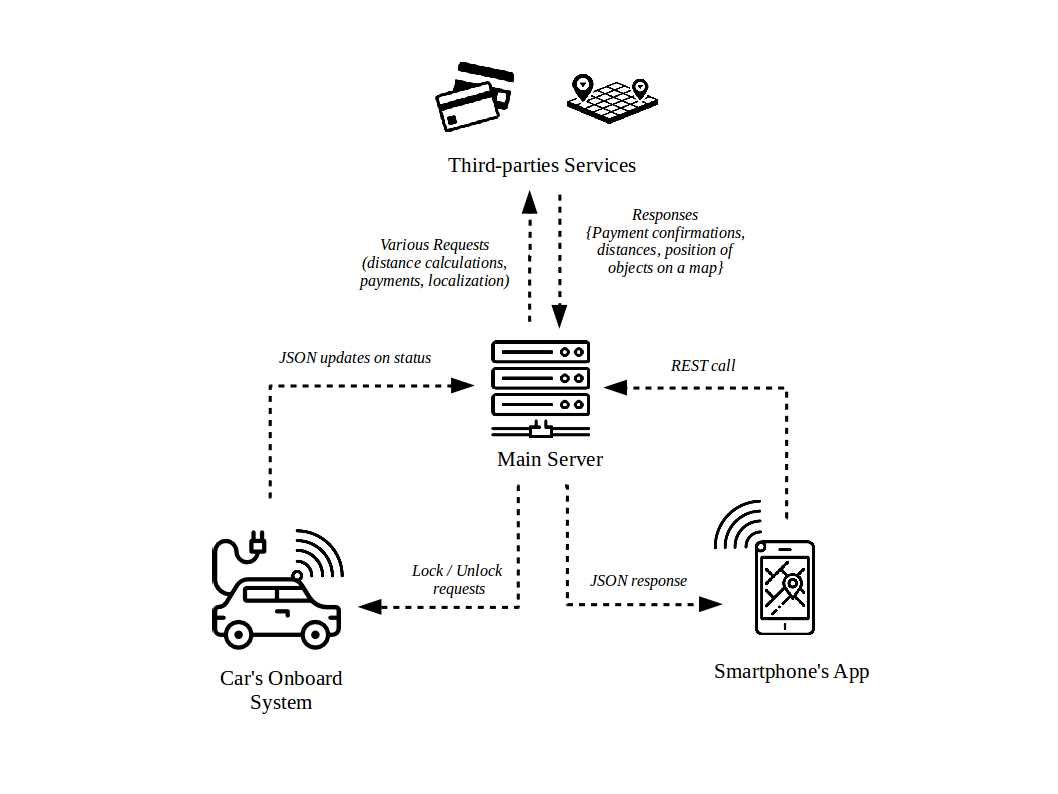
\includegraphics[width=1\textwidth]{proposed_system.png}
	\caption{High level overview of the architecture}
\end{figure}	

At this stage, the system's architecture is clearly two-tier:
\begin{itemize}[noitemsep]
	\item Tier 1, the main server, handles the application logic and data management.
	\item Tier 2, comprising mobile apps and cars, hosts the User Interface.
\end{itemize}

The system blends three different interaction models for each of the three pair of components interacting. In detail, we designed:
\begin{itemize}
	\item a pure \textbf{Client Server} approach when the main server interacts with the apps (customer's apps and staff's apps alike)
	\item a \textbf{Service Oriented} communication model between the main server interacting with external services like linf.io, truelicence.it, stripe.com etc.
	\item a \textbf{Publisher Subscriber} model between the main server and the cars' systems.
\end{itemize}

In subsequent sections we will provide more details about these components.

\subsection{Component View}

\subsection{Deployement View}

\subsection{Runtime View}
	\textit{ [Includes sequence diagrams to show how components interact to accomplish specific use cases]}

\subsection{Component Interfaces}

\subsection{Architectural Styles and Patterns}
	\textit{ [Explain patterns used above]}

\subsection{Other Design Decisions}


\newpage
\section{Algorithm Design}
	\textit{ [Definition of critical sections of code] }


\newpage
\section{User Interface Design}

\subsection{Mockups}
Mockups have already been included in the RASD (section 3.3: Non Functional Requirements) 

\subsection{UX Diagrams}

\begin{figure}[H]
	\centering
	\includegraphics[width=0.88\textwidth]{UML/UXDiagramPublicApp.png}
	\caption{UX Diagram of the interface of customer's application}
\end{figure}

\begin{figure}[H]
	\centering
	\includegraphics[width=0.88\textwidth]{UML/UXDiagramStaffApp.png}
	\caption{UX Diagram of the interface of staff's application}
\end{figure}	

\subsection{BCE Diagrams}

\begin{figure}[H]
	\centering
	\includegraphics[width=1\textwidth]{UML/BCEDiagramPublicApp.png}
	\caption{BCE Diagram of the interface of customer's application}
\end{figure}	

\begin{figure}[H]
	\centering
	\includegraphics[width=1\textwidth]{UML/BCEDiagramStaffApp.png}
	\caption{BCE Diagram of the interface of staff's application}
\end{figure}	
	

\newpage
\section{Requirements Traceability}

Considering we designed the system using a bottom-up approach, designed components maps in a straightforward way to the goals specified in the RASD. Hoever we provide an explicit mapping of the two.

 \begin{description}
 	\item[REGISTRATION] Users can register to \pe.
	\begin{itemize}
		\item Server: RegistrationController
		\item Customer's App: RegistrationView (?)
	\end{itemize}

	\item[LOGIN] Users can login to \pe.
	\begin{itemize}
		\item Server: LoginController
		\item Customer's App: LoginView (?)
		\item Staff's App: LoginView (?)
	\end{itemize}

 	\item[LOOKUP] Users can find cars nearby a given position, it could be its position or a point in the map.
	\begin{itemize}
		\item Server: CarsLocation
		\item Customer's App: CarsView (?)
	\end{itemize}

 	\item[BOOK] Users can book a car for a short amount of time.
	\begin{itemize}
		\item Server: BookingController
		\item Customer's App: BookingView (?)
	\end{itemize}

 	\item[UNLOCK] When users are in proximity of the car they booked, the system can unlock it.
	\begin{itemize}
		\item Server: CarLockController
		\item Car: LockController
		\item Customer's App: CarNearby (----------------- SEE ISSUE #14)
	\end{itemize}

	\item[RIDE] Users can drive to their destination.
	\begin{itemize}
		\item Server: AuthDriver
		\item Car: LicenceScanner, EngineController, MQTT publishers, CarGUI
	\end{itemize}

	\item[SAFE\_AREAS] Users can locate safe parking areas.
	\begin{itemize}
		\item Server: AreasLocation
		\item External Services: linf.io
		\item Car: MQTT publishers, CarGUI
	\end{itemize}

	\item[UNSAFE\_PARKING] The system must react to an unsafe parking.
	\begin{itemize}
		\item Server: UnsafeParkingController, IssuesController (?)
		\item Car: EngineController, LockController (MQTT publishers too?)
	\end{itemize}

	\item[POWER\_STATIONS] Users can locate charging stations.
	\begin{itemize}
		\item Server: AreasLocation
		\item External Services: linf.io
		\item Car: CarGUI
	\end{itemize}

	\item[CHARGE] At the end of the ride, users are charged a fee.
	\begin{itemize}
		\item Server: BillingController
		\item Customer's App: PaymentDetailsView
	\end{itemize}

	\item[PAYMENTS] Users can pay bills through the app.
	\begin{itemize}
		\item Server: PaymentController
		\item External Services: stripe.com
		\item Customer's App: PaymentDetailsView
	\end{itemize}

	\item[FIND\_ISSUES] The staff can locate cars that need their intervention.
	\begin{itemize}
		\item Server: IssuesLocation
		\item Staff's App: IssuesView (?)
	\end{itemize}

	\item[SUPPORT] The staff can identify and solve car's issues.
	\begin{itemize}
		\item Server: IssuesController
		\item Staff's App: IssueDetailsView (?)
	\end{itemize}

	\item[FINES] The system can provide enough details for the staff to manage correctly the fines they receive from local authorities.
	\begin{itemize}
		\item Server: FindDriverController (?)
		\item Staff's App: FindDriverView (?)
	\end{itemize}

 \end{description}


\newpage
\section{Conclusions}

\subsection{Tools used}
During the development of this document we used the following tools:
\begin{itemize}
	\item \textbf{Github} to version control the project
	\item \textbf{\LaTeX} on TeXworks to redact this document
	\item \textbf{www.draw.io} to draw UML graphs
	\item \textbf{Gimp v.2.8} to mockup the application
	\item \textbf{LibreOffice Draw} to draw the system's overview at section 2.1
\end{itemize}

\subsection{Hours of work}
\begin{itemize}
	\item SZ: 1h on 30/11
	\item SM: 5h on 2/12
	\item SZ: 5h on 2/12
	\item SZ: 3h on 5/12
\end{itemize}


\end{document}  

%%%%%%%%%% PARTE VECCHIA QUA SOTTO %%%%%%%%%%%%%%%%%


\subsection{Proposed System}

The proposed system features a client-server architecture, so it is divided into two parts: a frontend app for smartphones, which allows the users to use the service, and a backend system wich deals with all the operations and coordinates them. The backend also interact with the cars, that can be seen as a third part of the system.

\begin{figure}[H]
	\centering
	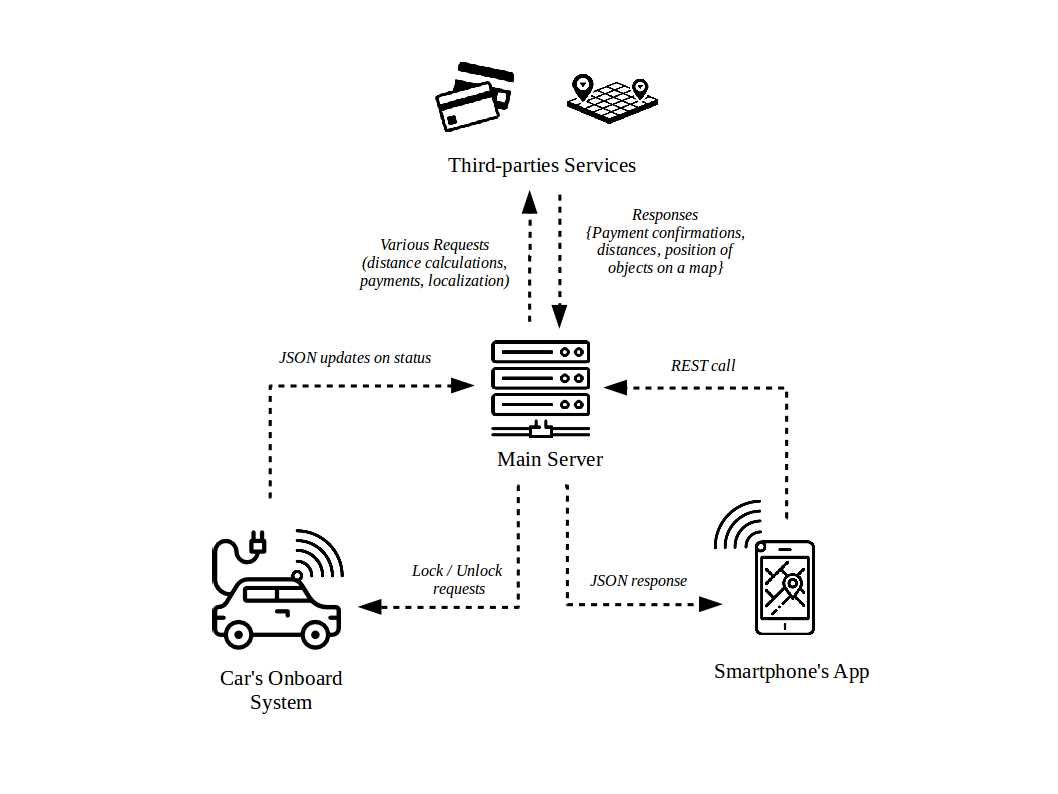
\includegraphics[width=1\textwidth]{proposed_system.png}
	\caption{Description of the proposed system.}
\end{figure}

\subsubsection{App Frontend}
The frontend is a thin app that relies on the smartphone's internet connections in order to work. Almost no operations can be performed with the app alone: all transactions are sent to the main server first, then processed and the result sent back to the app.

The app can be classified as a thin client.

\subsubsection{Centralized Backend}
The backend is the core of the system. Being able to process a lot of parallel operations, it can deal with all the requests coming from che clients ina reasonable amount of time (see Non Functionals Requirements). The backend is based on an MVC architecture and a REST API.

\subsubsection{Car's Onboard system}
The cars are equipped with an onboard system that monitors the status of the car, its location, and can send all the necessary informations to the main server. There won't be direct interactions between the car and the user's app.


